% Created 2017-02-04 Sat 21:17
\documentclass[11pt]{article}
\usepackage[utf8]{inputenc}
\usepackage[T1]{fontenc}
\usepackage{fixltx2e}
\usepackage[]{graphicx}
\usepackage{longtable}
\usepackage{float}
\usepackage{wrapfig}
\usepackage{rotating}
\usepackage[normalem]{ulem}
\usepackage{amsmath}
\usepackage{textcomp}
\usepackage{marvosym}
\usepackage{wasysym}
\usepackage{amssymb}
\usepackage[hidelinks]{hyperref}
\tolerance=1000
\usepackage[lf]{ebgaramond}

\usepackage[style=authoryear,natbib=true,backend=biber,firstinits=true,hyperref=false]{biblatex}
\bibliography{./../biblio/bibliography}

\author{Henrik Frisk \thanks{With acknowledgments to my collegue and
    friend Anders Elberling who has contributed immensely to this project.}}
\date{\today}
\title{Machinic propositions: Developing artistic ideas through conceptual deduction and improvisation}
\hypersetup{
  pdfkeywords={},
  pdfsubject={},
  pdfcreator={Emacs 24.5.1 (Org mode 8.2.5h)}}
\begin{document}

\maketitle


\section*{Introduction}
\label{sec:introduction}

One of the great promises of artistic research is the way in which it
allows for an insight into the inner workings of artistic
practices. Given an appropriate methodology, the researcher may tap
into the processes that lead up to the artistic work or the
performance. Although other research fields, such as art history,
musicology, ethnography along with many others, have also shed light
on these processes  of artistic production, what makes
artistic research both challenging and interesting is the double role
played by researchers/artists while exploring their own practices.

% In this chapter, however, the objective is not solely to make the artistic practice available for research, and, furthermore, not all artistic practices are possible to research.

The particular focus in this paper is to discuss methods that have
been developed in the duo \emph{Mongrel}, the members of which, Anders
Elberling and I, have worked together for several years on
numerous intermedia projects.\footnote{Our first artistic
  collaboration started in 2010.} I will attempt to show examples
of the impact artistic methods may have on the way an artistic
practice unfolds over time. In artistic research or research focused
on artistic practices, it is not uncommon that the research also
introduces a change both into the practice and in the
artist/researcher. In fact, this may be seen as a feature of artistic
research. In an article from 2013, Stefan Östersjö and I describe this
change as one of the core values of artistic research and we argue: 

\begin{quote} [\ldots] for the need to approach artistic research from
  an experimental perspective, not as a stylistic measure but as a
  quality in the artistic aims. A core value in artistic research is,
  as far as we know it from our own work, the possibility to amplify
  artistic processes that aim at creating a change in one’s own
  practice, a change that, when it is described and thoroughly
  documented, can effectively communicate new
  knowledge. \citep[][p. 27]{frisk-ost13}
\end{quote}

That changes in the processes that lead up to an artistic work may
change the outcome may not come as a surprise. What is remarkable,
however, is rather the opposite. The extent to which the artistic
\emph{work} in Western culture is often still seen as an immutable
object and the product of one single originator is striking. Even
relatively distributed artistic practices such as film production is
often referred to as the work of a director. The perspective of the
originator is guiding the apprehension of, and also, to some extent,
the understanding of the work of art. In this view it is the stage 
director at the theatre rather than the actor, and in the concert hall it is the composer of the music played by
the symphony orchestra rather than the musicians that play it that is
the point of reference, only to mention two examples. For other fields, the configuration of the
agents involved may be of a different kind, but the dominance of the
view of the artwork as the result of one single originator is not to
be mistaken, especially in music.

There is, however, several indications that this view is slowly
changing. In 2005, with reference to Lydia Goehr's important work
\emph{The Imaginary Museum of Musical Works} Georgina Born theorized
the changing ontology of music to open up for ``an approach that
incorporates understandings of the social, technological and temporal
dimensions of music'' \citep[p. 8]{Born2005}. She points to several
important aspects of this development relating to, among other things,
the destabilizing effect that music in itself may have on common
dualisms such as those between
subject and object, and production and reception, and through the
analysis of three different examples of digital creativity she continues:
\begin{quote}
  The aim is to show how we can use these tools to conceptualize
  changing forms of musical creativity, which themselves evidence new
  music ontologies that became ascendant over the course of the
  twentieth century. Taking three examples in which music is engaged
  with digital technologies and which evidence new kinds of creative
  process, I develop concepts of relayed creativity and of the
  provisional work. Throughout, key motifs are mediation, creativity,
  and the negotiation of difference.

  These perspectives reveal music to be a medium that makes mutable
some of the central dualisms of Western metaphysics: the separation of subject from object,
authentic from artificial, present from past, individual from collectivity. Routinely, as I have
indicated, music forms hybrids and transitions between these ‘pure’ states. In the face of such
complexities, it is unhelpful to divide the study of music itself from the study of its social,
technological and temporal forms.
  \citep[p. 8]{Born2005}
\end{quote}

This resonates well with some of the ideas proposed in this paper. Through artistic practice and consistent artistic methodology, the rigid conceptualization of music as an object rather than an activity may be questioned.


\section*{Mongrel}
\label{sec:mongrel}

In the duo \emph{Mongrel}, the overarching ambition is to critically
examine the nature of the relationship between auditory and visual
elements in intermedia works. Our works have been performed in the
United Kingdom, Denmark, Sweden, Belgium, Germany, and Vietnam. Our
most recent project, \emph{Machinic propositions}, is simultaneously
an artistic project and an attempt to critically examine Deleuze and
Guattari's theorems of deterritorialization as found in chapter seven
and ten of their seminal work \emph{A Thousand Plateaus}
\citep{deleuze80}. The output has taken a few different shapes and
has been using different kinds of media such as text, live
performance and fixed media
format. Like much of our other works \emph{Machinic propositions} is
part of the attempt to counteract the predominance of one medium over
the other, in particular, video over audio, which is not to say that we necessarily
strive for their integration into one another. Instead the ambition
is to allow one to become the other under certain conditions,
comparable to what is described by Deleuze as ``not an exchange, but
'a confidence with no possible interlocutor' [\ldots]; in short, a
conversation'' \citep[p. 2. The quotation contains an unspecified reference.]{deleuze77}.

Furthermore, there are parallels between the way we work,
and the idea, put forward by Deleuze, of style as the ability to
``stammer in one's own language'' \citep[p. 3]{deleuze77}. Our working
process is, like any other artistic process, situated in our personal conditions and
flaws but in \emph{Machinic Propositions} we specifically use them to
gain access to the ability to the ability to stammer in
language while avoiding it in speech,
metaphorically speaking \citep[p. 3]{deleuze77}. Among other things,
in practice we weave in Elberling's dyslexia and use his
misreading of the text as concrete material in the process allowing
new meanings to rise from the mistakes.

Different modes of synchronization between sound and video, and the wish to compose their
relations have become central to our work. There are nevertheless many
points of entry. With his highly influential work in electro acoustic music
Michel Chion has written extensively about sound in film. In his book \emph{Audio-Vision. Sound on
  Screen} he describes two different ways in which music in film can
evoke particular emotions in relation to what is seen on screen. The
first, \emph{empathetic music} is closely linked to the events in the
film. It follows the same rhythm and pacing, is phrased along with the
actions and is coded as being happy or sad along with the plot on
screen. A rather different approach is when music is juxtaposed onto
of a film scene and serves as a backdrop that intensifies emotion in a
manner that may ``exhibit conspicuous indifference to the situation''
\citep[p. 8]{Chion1994}. Examples of \emph{anempathetic music}, as he
calls this latter type include ``musical bits from player pianos,
celestas, music boxes, and dance bands, whose studied frivolity and
naivete reinforce the individual emotion of the character and of the
spectator, even as the music pretends not to notice them''
\citep[p. 8]{Chion1994}.

In the project \emph{Machinic propositions}, we instead look at the
relation between the two media as a system of de/re-territorialization
as described by \citet{deleuze80}. In this we way we were able to
depart from the empathetic/anempathetic view proposed by Chion and
attempt to detach both sound and image from their highly defined modes
of engagement. Following this we then examine the ways in which the
actual relations may be re-established within our systems of working,
using a range of approaches. Another way through which we experiment with
these topics is to change roles in the work and performance
situation. When I as a musician have to surrender the
control of the music to Elberling, primarily a video artist, and he
does the same to me the relations and the attitudes towards the
material are bound to change. This is to some extent a question
of creating usable interfaces for one another, but the actual
situation also changes our respective understanding of the practice
that we are engaged in consistent with our core ambition to
deconstruct the relationship between sound and image.

Concerning the theorems of deterritorialization there are some
interesting and immediate observations that may be done relating both
to the challenges in combining audio and video as well as to our
particular practice. For instance theorem two quite literally has
some bearing on the factual reality of digital sound and image: ``The
fastest of two elements or movements of deterritorialization is not
necessarily the most intense or most deterritorialized.''
\citep[p. 193]{deleuze80} The update rate of digital audio and video
is in the region of 1764/1,\footnote{This obviously depends on the
  sample rate and the frame rate respectively.} yet video is commonly the dominant medium
in this relation (though audio has its advantages sometimes) which
possibly points to the relevance of this particular theorem in our work.

Our practice, as will be further described below, as many other
practices, is perhaps to be likened to a rhizome, a network of ideas
that is, in the beginning, spread out on a plane, not randomly, but
unorganized. The nodes representing these ideas are highly distributed
in both space and time. Eventually, through the work processes and the
conceptual development, a folding of this space is taking place, and
virtual wormholes are created between nodes that in the beginning may
have been located far from each other but which now become
connected. This is to some extent a self-organizing process that finds
some resonance in \emph{A Thousand Plateaus}. In the opening chapter, by reference to
\citet{rosenstiehl974}, \citeauthor{deleuze80} comment that to:

\begin{quote}
  these centered systems, the authors contrast acentered systems,
  finite networks of automata in which communication runs from any
  neighbor to any other, the stems or channels do not preexist, and
  all individuals are interchangeable, defined only by their state at
  a given moment—-such that the local operations are coordinated and
  the final, global result synchronized without a central
  agency. \citep[p. 19]{deleuze80}
\end{quote}

However, before continuing the discussion on the methods we use I will
return to some of the work that proceeded \emph{Machinic
  Propositions}. In 2014-2015 we started a project called \emph{The
  Image Illiterates} with the outspoken intention to explore the
possible relations between audio and video in the kind of audio/visual
work that we are interested in. The project was a result of
observations we did in 2013 while working on the video installation
\emph{Elle a dansé, Il se tourna} (see Figure \ref{fig:orpheus-1}) concerning
audio/video synchronization.

\begin{figure}
  \label{fig:orpheus-1}
  \centering
  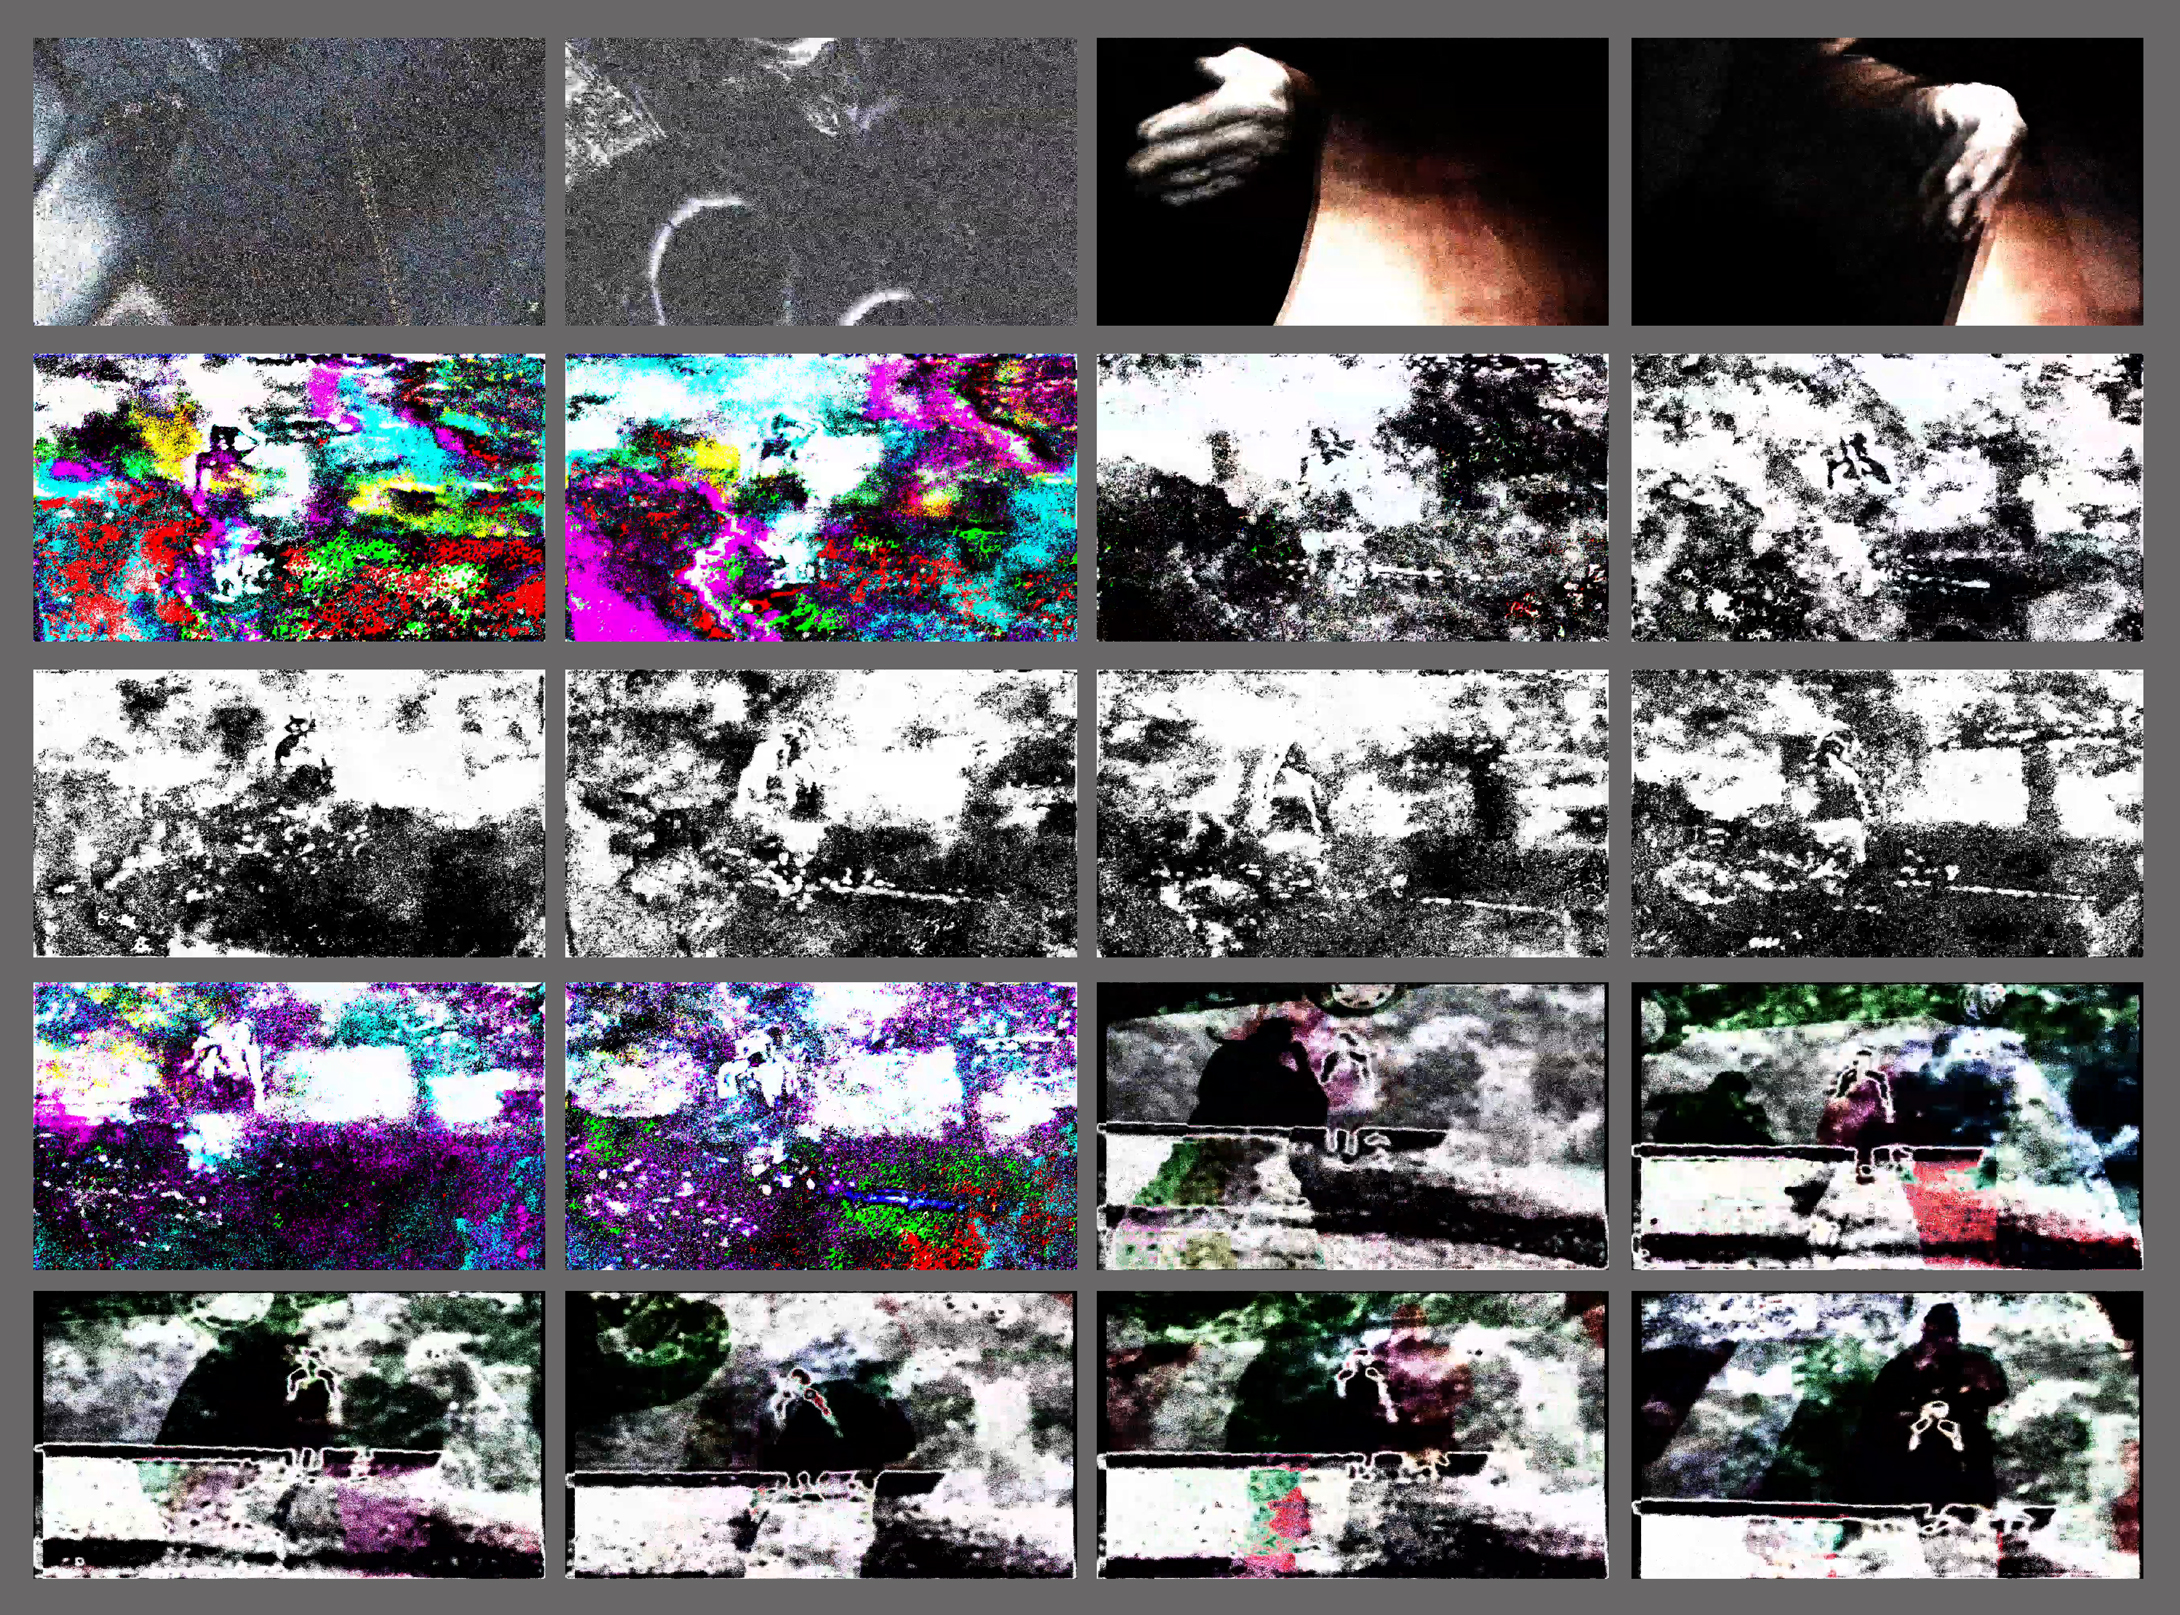
\includegraphics[width=\linewidth]{img/orpheus-1.jpeg}
  \caption{Excerpts from \emph{Elle a dansé, Il se tourna}}
\end{figure}
In a preliminary conclusion of \emph{The Image Illiterates}\footnote{The project was first presented publicly at the symposium \emph{Tacit or Loud: where is the knowledge in art?} in Malmö, November 28 - December 3, 2014 (http://www.teatrweimar.se/tacitorloud/find.htm)} in March 2015, we wrote in our work diary that:

\begin{quote}
  to work on modes of synchronization is possible, but at the same time it is impossible to draw any general conclusions from the work we have done so far: whatever knowledge comes out of this becomes useless in other contexts. Sound and image are essentially different, they operate in different dimensions. What we uncovered, however, was that the solution lies rather in the attempt to move away from trying to synchronize the perception of sound and video, and instead focus on common processes that bind the elements together. (\emph{project diary, translated from Swedish by the author, March 11, 2015})
\end{quote}

What we point to here is what we felt was a necessity of a development
from temporal synchronization between individual elements in the video
and audio respectively towards a more process-oriented approach to
synchronization. In the different version that we have hitherto
produced of \emph{Machinic Propositions} an example of this may be
found. The opening two and a half minutes features a transformation of both audio and video from very noisy
sound and pixelated video to smooth sound and image. This is a very simple
transformation that in effect merely increases the resolution of both
media in parallel (see Figure \ref{fig:machinic-1}). In this segment there is not much temporal
synchronization on the level of events, instead, we delegate the
synchronization to the process. The result is that sound and image are
woven together, not as one, but in dialogue: both speak the same
'language' but use different 'words'.

\begin{figure}
  \centering
  
\includegraphics[width=\linewidth]{img/stills-compilation-beg.png}
  \caption{Screen dumps from the opening of \emph{Machinic propositions}. The video is continuously processed from very low resolution to very high matched by a similar alteration of the audio.}
  \label{fig:machinic-1}
\end{figure}

What we also discovered in the project \emph{The Image Illiterates}
was the asset of focusing our attention on the artistic process and the
result as a whole rather than on the idea that one is leading to the other. The most
important empirical data in this project are the improvisations
we did together. Departing from a sketch or a rough framework, we went on to
set up a small set of instruments independently of each other that we
could play. Then we improvised together, generating material in real
time after which we spent much time analyzing what we had achieved. Feedback
between these instruments, that is, data fed from one instrument in
the audio domain to another instrument in the video domain and vice
versa was also an important aspect. The outcome of the improvisation was often
satisfactory on the level of the integration of the different
materials, and in the sound and video interaction specifically, but
with relatively few post-improvisation manipulations the result was
significantly improved in nearly all cases
compared to those where we had tried to
structurally synchronize the events in the improvisation. This aspect
of the work is discussed in more detail below. 

Artistic work is to a large extent a practice that takes
place in a material reality, even if the perception of such actions may
approach the virtual.\footnote{According to Deleuze's definition of
  the virtual, however, artistic practice the way we see it may perhaps
  be virtual in essence \citep[See e.g.][]{deleuze88}.} In music, the
practice often needs time to develop--although some processes are
better developed out of time. Nevertheless, the way Deleuze and
Guattari talk about the rhizome as ``a map and not a tracing''
\citep[p. 13]{deleuze80} is, at least for the work method we have
developed, both a fitting description and a useful mode with which to further
develop our processes. Mapping the patterns we are creating, our
individual as well as each other's, is a process that may be
seen as the attempt to reduce the number of possibilities in our
project, while at the same time attempt to increase the number of
possible connections. As can be seen in the short excerpt from our
work journal we had already started moving in this direction and it
was about this time that the idea of doing a project on the theorems
of deterritorialization first materialized. 

Through the theorems of \emph{A Thousand Plateaus} we began to work
out an abstract intermedial work trying to maintain a critical
attitude towards the philosophy of Deleuze and Guattari specifically
and the very notion of using philosophy as the input to artistic
processes. With the use of the theory we further developed our
conceptual tools, and more specifically, the way we use our senses
\emph{see} and \emph{hear} in the way we tackle the theory
participates in creating a zone of relative freedom that can provide
possibilities for a new understanding of what we do as artists and
researchers.

\subsection*{Conceptual deduction}
\label{sec:conceptual-deduction}

Our artistic method is one where narrative and improvisation play central
roles. It has grown out of our thinking about contemporary media and
our attempts to critically examine both our own pro-technical
approach, and the hypermedia landscape we act and live in. The method has
been developed based on our artistic ideas, the needs of the projects
we engage in, and the conditions of our respective practices. Our process is slow
and meticulous. The work on \emph{Machinic propositions} began in 2015
and is likely to continue for another few years. In other words, the
actual artwork only materializes at the very end of a relatively long
process of interaction, and after that, it may continue to develop
through numerous iterations. However, the work in itself in terms of a
resulting performance is in this
context less important than the process to the point where there is
almost a reversal of the two terms: the work is the process and the
work is simply one out of many possible parts of the process. 

The method of conceptual deduction may be related to a variety of
contexts and may primarily be associated with scientific research and systematic inquiry perhaps not
commonly referenced in the context of artistic research. In Monrad Rrenban's book
on the early works of Walter Benjamin, he writes that ``Benjamin
suggests the practice of philosophy is not the conceptual deduction
(deduction into concepts) of research but is also somewhat distinct
from the metaphorical determinateness [\ldots] in the artwork''
\citep[p. 117]{rrenban2005}. For us, however, both the metaphorical
determinateness and the conceptual deductions are part of the
formative movement towards a performance. In \emph{Mongrel} we
are using it freely, and mainly as a tool to reason our way through the
constructive phases of our artistic practice. In some ways this is not
so different from using improvisation as a method as improvisation may
also be concerned
with creating models that contribute to bringing negotiation of
the material forward. Hence, it is a process in
which we align and synchronize the general ambition of the work and,
perhaps most importantly, it brings differences in our respective
aesthetics to the surface in a way that is useful to us. We may start with an existing story, a
fictional character or a philosophical text, but we may end up with
something quite different. Being as it is artistic
practice, the goal of the method is not necessarily to gather information --
although this could very well be one of the results. Instead, it is about
creating a performative platform that we share and that we later use
to guide the development of material for our works. 

It is a time-consuming process the strength of which is not always
evident in the practice and it can lead to the kind of pivotal moments
where the entire structure needs to be rethought. As was mentioned,
the basic premise of the method, the way we use it, is that we start
with a general story or concept that we explore together.  For the
work \emph{Elle a dansè – Il se tourna} \citep[][]{mongrel2013} we
explored the legend of \emph{Orpheus and Eurydice}\footnote{\emph{Elle
    a dansè – Il se tourna} was commissioned for the project \emph{Go
    to hell} and was premiered in Stockholm in October 2013.}. Through
a process in which we studied various interpretations of the legend,
dissected its parts, applied different perspectives on it and, more
than anything, discussed it with each other, we slowly created a
framework that served as a virtual space for our collaboration. This
conceptual framing \citep[][p.199-201]{Olofsson2018} goes beyond a
mere collection of relevant references and its primary goal is to
provide us with conceptual tools, and a language with which we are
able to negotiate the creative processes.

In \emph{Elle a dansè – Il se tourna} we ended up constructing the
piece upon only one single scene in the legend of \emph{Orpheus and
  Eurydice}: the moment where Orpheus rises from Hades with the
promise that Eurydice would be brought back to life provided he would
not look back before he had returned into the real world. In the last minute before coming out
into the sunlight he loses his faith and turns around to make sure
that Eurydice was still there. The process
that led us to the decision of working with only this isolated part of
the story was informed by conceptual deduction but also by the
particular conditions for our practices as well as technical
considerations. In other words, it is rarely \emph{one} method or \emph{one single
aspect} of a methodology that provides all of the necessary material,
but the different methods used makes it possible for many different,
and sometimes unexpected, aspects of the practice to surface.

We use the same method on the theorems of deterritorialization by
\citeauthor{deleuze80} in \emph{Machinic propositions}. For example,
it was theorem two (was cited above) that led to the idea of applying
a simultaneous
process of resolution increase of both sound and video. In the
beginning it was mostly an experiment if the theory actually held
true, if the speed of the elements is not a deterritorializing
factor. 
%I will first give a theoretical background to the 

%%%%%%%%%%%%%%%%%%%%%

\subsection*{Intermediality}
\label{sec:intermediality}


For a preliminary discussion on the challenges concerning the way we
use different media in our work, I will use the
theoretical framework developed by \citet[][]{Ellestrom2010}. This paper is
not the place for an in-depth analysis of all the different facets of
the broad field of media studies and the introduction here is just a
scratch on the surface to allow for a discussion on the different
strategies we have developed in \emph{Mongrel}.

\citeauthor{Ellestrom2014} states that broadly, ``media may be
understood as communicative tools constituted by related features. All
media are multimodal and intermedial in the sense that they are
composed of multiple basic features and are understood only in
relation to other types of media'' \citep{Ellestrom2014}.  Both of the
two primary media we work with in \emph{Mongrel}, 'video' and 'music',
are \emph{qualified media} signified by the fact that they are
``characterized by historical, cultural, social, aesthetic and
communicative facets'' \citep[p. 5]{Ellestrom2010}. Different kinds
of media are commonly both very different from each other while
at the same time they may exhibit great similarities, and for this reason
``intermediality must be understood as a bridge between medial
differences that is founded on medial similarities''
\citep[p. 12]{Ellestrom2010}.

As is pointed out by Christina Ljungberg ``intermediality also
displays degrees of self-referentiality''
\citep[p. 88]{Ellestrom2010-CL} and this aetheticized quality is both
an asset and a problem for us. The moving image on the screen has
become such an icon in and of itself in the Western culture. The
general spectator is so accustomed to sound and image being one
unified, or qualified, medium to the point where it gets difficult to
challenge this unity. Since one of our objectives in \emph{Mongrel}
was to critically examine the relation between audio and video it
became necessary to address the fact that film, as in moving image and
sound, is commonly understood as one discrete medium, or art form. Or,
as \citeauthor{Ellestrom2010} puts it, ``there is a strong tendency
towards treating a medium as \emph{a} medium, or an art form as
\emph{one} form of art, only when certain qualitative aspects can be
identified'' (p. 25). In a manner of speaking, the film component
consumes the music and constructs a single aggregate that encompasses
both mediums. We were, however, interested in treating them separately
only to reconstruct, and to some extent shape, their intermedial
relation in the performance or in the composition of the material onto
a fixed media format.

But also, another factor that contributes ``to the
self-referentiality of digital art is the emphasis artists put on the
very process involved in producing art by more or less smoothly
integrating the various media into an intermedial whole''
\citep[p. 90]{Ellestrom2010-CL} which is directly related to how we
use our narrative method. It is through the relentless restructuring of the
conceptual framework, and the significant choices that we make based on
the conceptual deduction, that we attempt to model the conditions for
intermediality.

% \emph{intermediality} 
% and \citeauthor{Ellestrom2010} states that ``the understanding of what
% a medium is and what intermedial relations actually consist of has
% vital implications for each and every inquiry in old and new fields of
% study concerning the arts and media: ekphrasis, cinema, illustration,
% visual poetry, remediation, adaptation, multimedia and so on''
% \citep[p. 11]{Ellestrom2010}. This challenge is part of the core
% the difficulty in attempting for a definition of any of these terms
% but intermediality in particular.

% In an attempt to avoid the by all means impossible definition of what
% a medium is - a term that has a wide range of meanings attached to it
% that differ from field to field - \citeauthor{Ellestrom2010}
% distinguish between basic media, qualified media and technical media.

In our work the construction of intermediality between sound
and image is achieved in a number of ways. The ways in which the material is
conceptualized and aesthetisized, laid out and composed, and negotiated
and performed contribute to intermedial bridges being created. In \emph{Mongrel} I primarily work with 'my' medium,
sound, but I am responsible for composing the nodes that allow the
intermedial connections to the video to materialize. By composing the
music with an inherent interactive potential that Elberling may pick
up, the intermediality of the two mediums may be explored. In other
words, working with the sound themselves, the way they are structured
and with the way they may, or may not, interface with the visual
medium, allows me to contribute to the perception of sound and video
as two parts intermedially connected rather than sound and video
combined into one discrete medium. 

% In artistic practices that involve collaborative work of some kind the fact that some kind of change is introduced in the preparatory phases of the work also changes the work I imagine is a common experience.  



% Depending on where in the process the practice is currently
% operating. A simple example may be a short musical phrase the meaning
% of which may be completely different depending on who is listening and
% what the role this listener has in relation to the material. 



\begin{figure}\label{fig:impro-1}
  \centering
  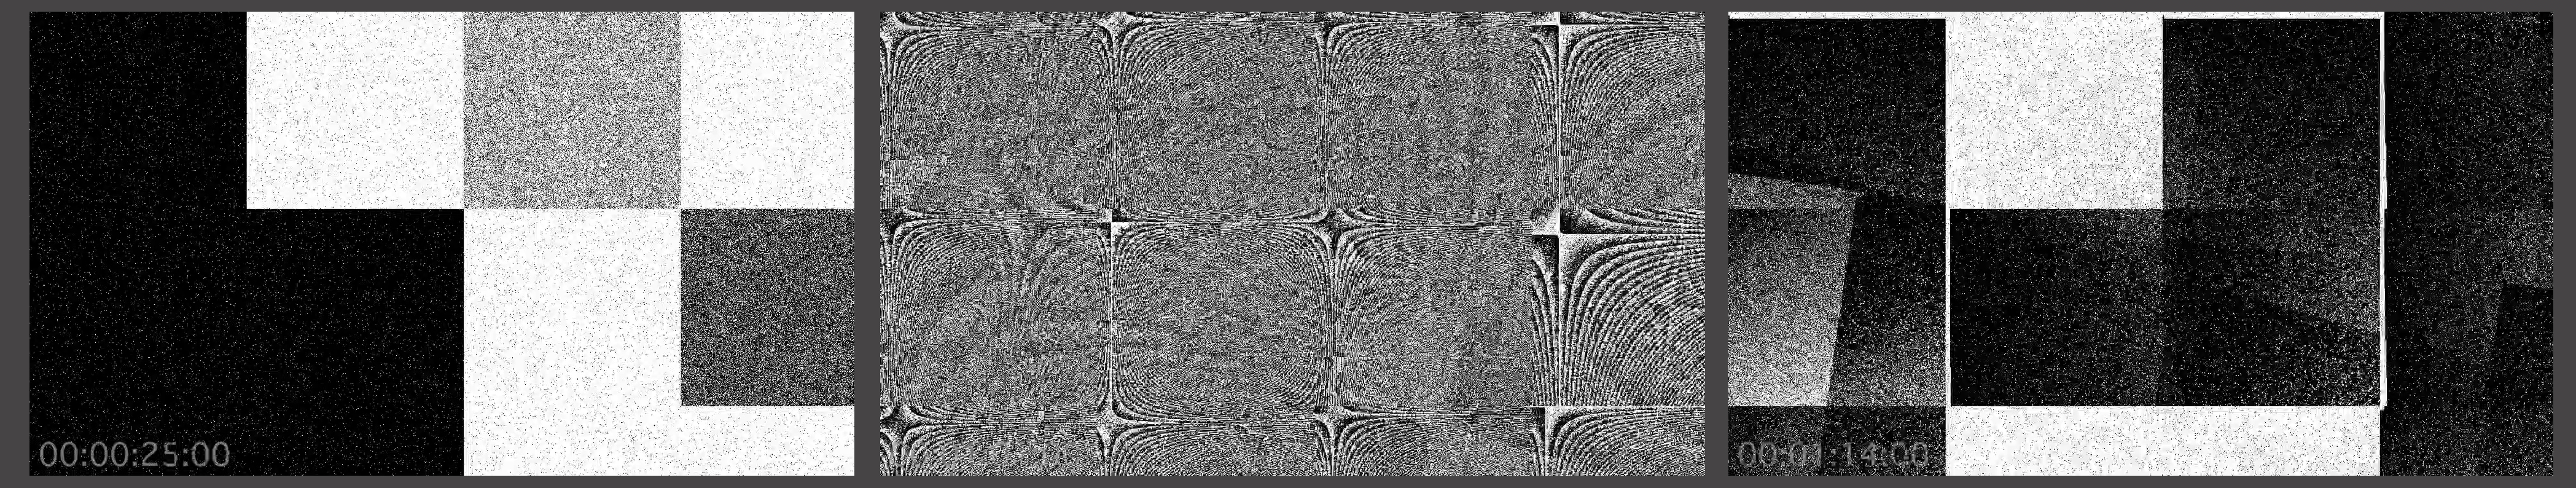
\includegraphics[width=\linewidth]{img/impro-1.jpeg}
  \caption{Screen dumps from a studio improvisation by Mongrel.}
\end{figure}

\section*{Performativity}
\label{sec:performance}

In the performing arts - and probably in most artistic and creative
activities - there is a distinction between the processes that lead up
to a performance and the perception and results of the
performance. This is not to say that they are isolated from each
other, nor that they do not overlap in several important ways, but
rather to point at the difference in the way the artistic practice is
perceived in these two modalities. As was mentioned above in
\emph{Mongrel} we have often noted the specific difference between how
we perceive what we do while improvising, and how we perceive it
listening back to it: within the practice, in the play mode, the
results have a slightly different meaning than what they have in an
analytical mode, outside of the performative practice. This is not so
surprising in itself, after all, there is a logic that belongs to
performance and a different kind of logic that comes with
listening. There are however two observations that I would like to
make here and that both have been important in our work. The first is
related to the way performance, or performativity, affects the
context, and the second relates to the different general qualities
that performances and compositions exploit. The former is discussed in
the following and the latter in the next section.

In a concert of instrumental music, I as a listener become a part of
the performance although, in contrast to, say, performance art and
more experimental performative genres, in a traditional concert space
some effort is made to separate the listener from the
performance. This is achieved both through the physical design of the
space (such as a high stage), as well as through social means
(e.g. particular rituals in the concert form). Nevertheless, the
physicality of the performance is more often than not a constituent
aspect of the perception of a concert, and looking at performativity
in this way, as something which goes beyond the activities of the
performer alone, has opened up for a new aesthetics and new ways in
which performativity may be understood. In her book \emph{The
  Transformative Power of Performance: A New Aesthetics} Erika
Fischer-Lichte describes this as the performative turn:
\begin{quote}
  The dissolution of boundaries in the arts, repeatedly proclaimed and
  observed by artists, art critics, scholars of art, and philosophers,
  can be defined as a performative turn. Be it art, music, literature,
  or theatre, the creative process tends to be realized in and as
  performance. Instead of creating works of art, artists increasingly
  produce events which involve not just themselves but also the
  observers, listeners, and spectators. Thus, the conditions for art
  production and reception changed in a crucial aspect. The pivotal
  point of these processes is no longer the work of art, detached from
  and independent of its creator and recipient, which arises as an
  object from the activities of the creator-subject and is entrusted
  to the perception and interpretation of the
  recipient-subject. Instead, we are dealing with an event, set in
  motion and terminated by the actions of all the subjects involved –
  artists and spectators. \citep[p. 23]{FischerLichte2008} 
\end{quote}

% This is no less true from the point of the performer and there does
% not even have to be an audience in order to stage a performance. As a
% performer I am obviously also a listener.
The performative turn has no doubt contributed
to the development of artistic research. \citet{Haseman2006}, in his
manifesto for performative research, raises concern about the development of
qualitative research methodologies as a heading that encapsulates
everything that is not quantitative research. He suggests a third category:
\begin{quote}
  Accepting the concern of traditional qualitative researchers about
  the ‘performance turn’, it is possible to argue that a third
  methodological distinction is emerging. This third category is
  aligned with many of the values of qualitative research, but is
  nonetheless distinct from it. The principal distinction between this
  third category and the qualitative and quantitative categories is
  found in the way it chooses to express its
  findings. \citep[p. 102]{Haseman2006} 
\end{quote}
In performative research, the practice that the performance is part of
is an integral part of the research object and not an optional
activity that generates the material for research. Following this the
practice and its performative qualities are not merely freeing the
artistic researcher from the structures of quantitative or qualitative research, it
genuinely presents a novel approach ``that holds that practice is the
principal research activity — rather than only the practice of
performance — and sees the material outcomes of practice as
all-important representations of research findings in their own
right'' \citep[p. 103]{Haseman2006}. 

Kathrin \citet{Busch2009} makes a similar claim in her overview of
the characteristics of artistic research as an emerging poetics of
knowledge. Art and theory, she claims, 
are two distinct practices, yet highly interrelated and interdependent
in a system of transferences: ``In this constellation, philosophy
neither brings the arts to the point nor does art sensualize
philosophical truths; philosophy serves a knowledge-based artistic
practice as a point of reference, similar, conversely, to how art
might affect theoretical practice.'' \citep[p. 1]{Busch2009} In a
critique not only of the natural sciences but of a traditional view of knowledge production itself,
she argues for a holistic view in which the separation of the creation of the objects from
their representations, the performance from the object and the act of
performing from the act of listening is avoided. Busch continues:

\begin{quote}
  In other words, in view of a steadily growing knowledge imperative,
  it is necessary to recall the theoreticians who refuse to restrict
  themselves to functioning as suppliers of knowledge, who view
  knowledge itself with great skepticism, and who see even their own
  theories as an inherent practice of knowledge criticism. On the
  basis of such skepticism about basing art on science that idealizes
  academic standards, an \emph{art or a poetics of knowledge} can emerge that
  questions the actual construct of the sciences. \citep[p. 5]{Busch2009}.
\end{quote}

In this context, experimental research methods and artistic experimentation
are interchangeable and complementary. They are both part of artistic
practices, also practices that are contextualized as artistic research,
and, as was mentioned above, this experimental attitude should be at the core of the artistic
research practice \citep[p. 42]{frisk-ost13}. The experimental
attitude in artistic research is, by all means, to be regarded an
asset but may
contribute to the fact that it is less apt at arriving at a
specific result in terms of its knowledge production than what other
kinds of research are. Or, as put by \citet{Busch2009} ``it must be
emphasized that knowledge generated through art cannot as easily be
brought to a precise point, as might be implied by the phrase 'art as
science' '' (p. 5). In this sense artistic research provides an
alternative method that engages with knowledge as practice and
practice as knowledge.

The performative turn opened up not only for the
social understanding of performance but also for its political
dimension and Judy Butler's work is of course central. Her 1988
essay \emph{Performative Acts and Gender Constitution} is obviously
concerned with gender acts and not artistic performance, and the
urgency of the topics she is discussing is quite different from those
of artistic practice, but this social dimension of also artistic
performance is one way in which the transformative potential of
artistic research may be constituted: ``If the ground of gender
identity is the stylized repetition of acts through time, and not a
seemingly seamless identity, then the possibilities of gender
transformation are to be found in the arbitrary relation between such
acts, in the possibility of a different sort of repeating, in the
breaking or subversive repetition of that style''
\citep[p. 520]{Butler1988}. Similarly, if the ground for the traditional
work identity is to be found in the repetition of romantic ideas about
artistic practice, then the possibility for a
performative transformation should be found in novel approaches,
experimentation and in a different kind of repeating that breaks with
the very idea of style. In this configuration there is a possibility
for all the different kinds of agents involved in artistic practice,
in the widest sense also including audiences, to become part in the
formation of the artwork.

\begin{figure}
  \centering
  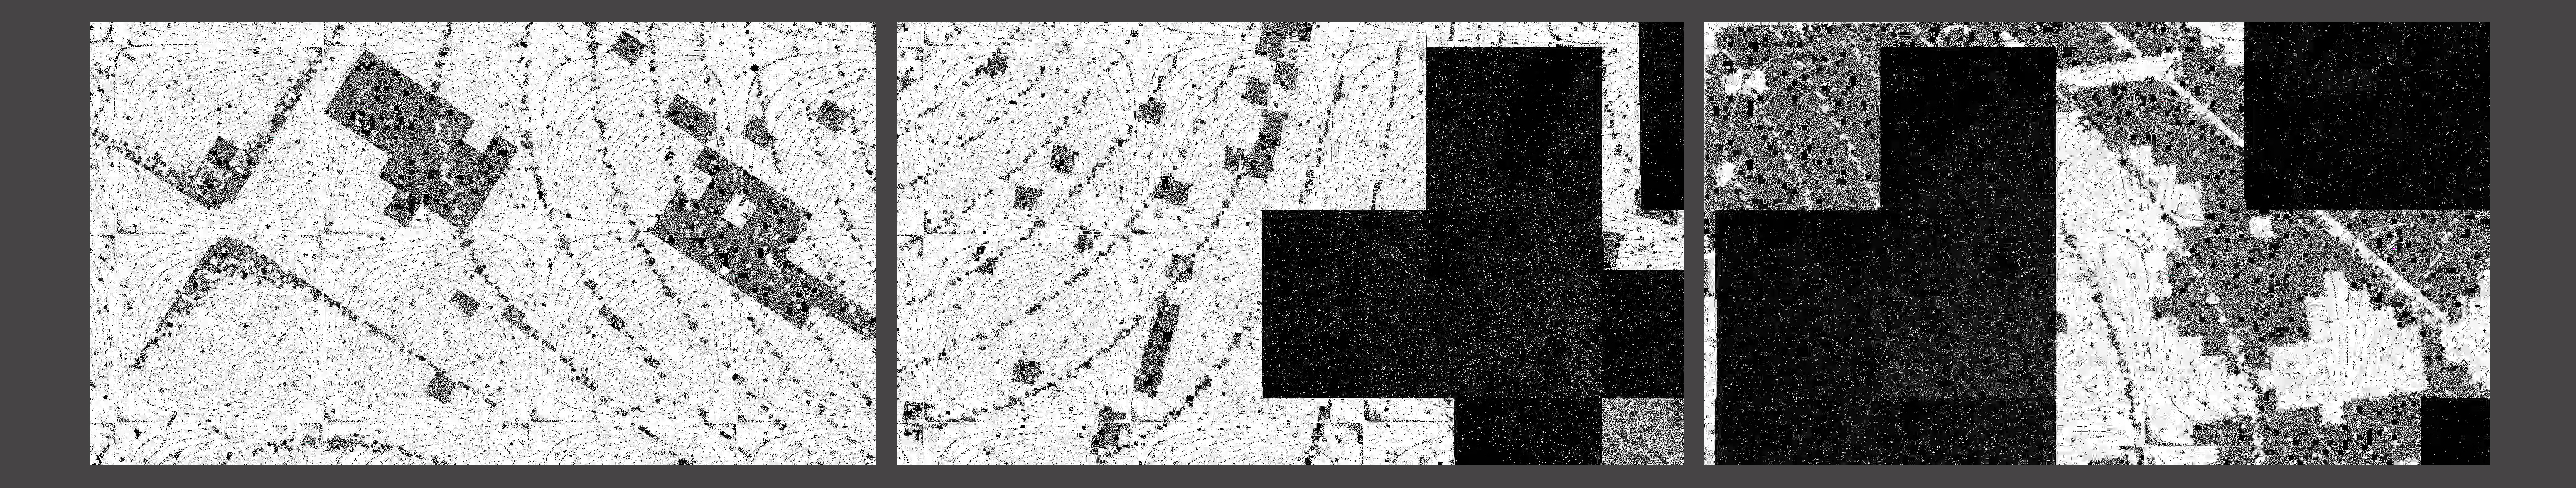
\includegraphics[width=\linewidth]{img/impro-2.jpeg}
  \caption{Screen dumps from an improvisation by \emph{Mongrel}.}
\end{figure}



\section*{Composition}
\label{sec:composition}

If the performance is the structuring of an event entangled with the
performer and the listener, perhaps a preliminary definition of a
composition, presumably mainly valid in the context of this paper, is the
organization of material in preparation for a performance. The
particular situation described above where we in \emph{Mongrel} would
improvise in the studio in order to generate material brings the
differences between the logic of performance and that of composition.

If we imagine that a live performance of an instrumental improvisation
is recorded and the recording is played back. Provided that the
listener has some contextual knowledge, such as of the instruments
played or the musical genre, the performativity may to some extent be
reenacted\footnote{There is some evidence to the fact that the
  physical experience of playing music effectively makes a difference
  for the listening. Neurological studies have shown that musicians
  respond physically when listening to music \citep[See
  e.g.]{bangert2003,overy2009}.} and the perception of the music is
that it is still primarily a performance, albeit a recorded
one. However, when the improvisation is done mainly by electronic means it may not have a
specific signifier with the result that the performative reenactment
may not take place or be difficult to invigorate. This is the
observation we did in \emph{Mongrel}: our improvisations had a very
different logic to them when performed than when listened to as if the
performativity of the improvisation was not encoded in the
recording. As a consequence, and as a consequence of also other reasons, we heard these improvisations as
compositions. Our assessment of the improvisations was generally more
positive based on our impressions during the performance than when we
listened back to them. This discrepancy between what it 'feels like'
in performance and what it sounds like listening back to it is
consistent with my experience ever since I started playing. What was
striking in this case, however, was that only very little had to be
altered in order to 'fix' the issues we had with the improvisation. A
few edits, primarily concerning the timing of events and the temporal
synchronization between the audio and the video was all that was
needed in order for the expression in the performance to work as a
non-performative piece, that is, a fixed media playback, or a
composition. This also meant that the improvisation changed nature
when it was recorded, from a performance to an improvisation
\emph{becoming} a composition. It is not uncommon that recordings of
performances are edited prior to release on CD for example, but one of
the points that may be made here is that the editing we did was mainly
concerned with the intermedial relations between the sound and the
video rather than the individual parts.

The differences in the perception of the performance that are tied to
the position of the perceiver have some
resonance in the difference between an actual performance and the
preparation for a performance.
The distinction between the preparatory activities and the
performative stage is more prominent in some fields of practice than
others. In musical composition, for example, the work of the
composer is often very different in nature from the work of the
musicians. A field in which these differences are often discussed is
in the field of game development or within the practice of 
constructing novel interfaces for musical expression, or the
design of software instruments. These practices are related to ours in
more than one way and we often design interfaces on which we can
play the pieces we compose. In our practice these interfaces are controllers of the
digital signal processing of audio and video but also interfaces to the other
medium: from sound to image or vice versa. For example, an interface that controls the pitch of some
synthesis algorithm may simultaneously control a visual filter in the
video, or, as in the example given above, one controller may
simultaneously control parameters in both sound and image. This approach is modeled on the necessity to
construct contexts for interaction both between the different kinds of
materials that we engage with, but also in order to bridge the borders
between the mediums involved in the work. However, the requirements
that shape an interface in the stage of composition may be somewhat
different from the needs proposed in the context of performance. This
is discussed by \citet{Nilsson2011} who points to the inherent aspect
of research and experimentation in the development of new instruments,
as well as to the specific interaction between the two phases:

\begin{quote}
As a point of departure, there is a mutual relation between activities at design time and activities at play time. In order to improve and to refine an instrument under development, analysis and evaluation of the perceived experience in play time became the basis for further activity at design time, which was followed by new experiments in play time, and so on.  In other words, in the reciprocal action between activities at design time and play time an instrument gradually takes shape. \citep[p. 25]{Nilsson2011}
\end{quote}

Even though the different processes overlap to a great extent, for the
performer the difference between design time and play time may be
perceived as fairly definite. In the organization of the material
something that appears perfectly logical may turn out quite different
in performance, and the repercussions of this perceptual difference
are quite real and sometimes unpredictable. The difference may be
described as the distinction between a constructive phase and an
interpretative, once theorized and specified semiotically by Jean \citet{molino} as
the esthesic and the poietic phases \citep[See
also][]{frisk-ost06-2}. In this model, both the producer and the
receiver are involved in complex processes that are far more
convoluted than a simple act of communication between two nodes. As a
performer, I can even be in both of these symbolic forms at the same
time and most musical improvisers have probably at some point
practiced the ability to evaluate and reflect upon that which one is
currently playing at the same time as one is playing. It is the
ability to listen to oneself with a critical ear as if one is located
outside of oneself while at the same time performing: respond
objectively to one's subjective playing. The
key aspect here is listening in the broad sense of the word, and
specifically, the ability to listen to oneself as well as to listen to
the other. 

Before moving on to the topic of listening, I will briefly
return to the notion of performativity. Barbara Bolt, in a comment to
\citet{FischerLichte2008} reminds us of the fact that the actual
listener/performer relation is disrupted through the performative
turn:
\begin{quote}
  In this performative turn, the nature of the relationship between
  subject and object, observer and observed and artist and audience
  has been refigured to create a dynamic and transformative
  event. There is no separation between the production and work, and
  the audience becomes part of the work. \citep[][p. 2]{Bolt2009}
\end{quote}
\citeauthor{molino}'s model is definitely structured around the idea
of a separation between the listener and the performer and the actual
object in this communicative transaction is in some way independent of
these processes (referred to as it is as the \emph{neutral}
level). Through performance, the relations between play time and design
time, as well as the separation between
construction and interpretation are being destabilized. This points to the necessity of using experience and practice from the
phase of play time in the process of design time, and the method that
allows for the seamless transition between the different stages is listening.

Briefly mentioned earlier in the context of developing ones ability
to listen to oneself as if one is located outside of oneself, the
invitation to \emph{listen} to the other should not reduce the
importance of listening to oneself. When we listen, what is it we
allow ourselves to be influenced by, and what part of our own
expression, if any, should remain untouched by our listening? How do
we resonate to the other and how do we respond to
resonance?\footnote{Resonance is a key word in \citet{nancy2007} book
  on listening.} There are no general wrongs or rights in listening,
only intuition and sensibility and at some point, there may be a
demand for absolute and unconditioned control, and at another, it may
be necessary to completely give in to the wish of the other. An ethics
of listening may guide an ethics of artistic research. The
romantically constituted and mythical artistic self is not always
useful in a research context and the dismantling of its mysterious
nature is an important, and perhaps even necessary activity in
artistic research.\footnote{The meaning and impact of the self as a
  central activity in artistic research is further discussed in
  \citet{frisk12-improv}.}


\section*{Discussion}
\label{sec:discussion}


As was discussed above even without an audience in a studio
improvisation, the difference between the modes of perception in
different stages of the artistic practice may come into play quite
noticeably. I find it remarkable how different a given improvisation
may feel depending on the listening context, but whether or not this
finding may be generalized and applied to other fields or studies is
very difficult to state. However, this is somewhat of an ill posed
question. That a given result is a finding with a high degree of
specificity is clearly not to say that they are uninteresting, nor is
the fact that one mode of knowledge production is not compatible with
another not a reason to dismiss it, as was alluded to by
\citet{Busch2009} above. Also unique and individually situated
knowledge is of interest in artistic research given that the methods
are relevant to the context. Artistic approaches, on the other hand,
may be easier to generalize and the continuous iterations of
practice-reflection feedback loops and, along with them, the
theory-method interactions that may surface as a result, are among
some of the most interesting aspects of artistic research to me. These
may involve transgressing the borders between preparation and
performance, between design time and play time and, between different
media. In these border crossings, there is an opening for a radical
and experimental research practice that has social as well as
political connotations.

For the musician to go beyond the purely musical realm and consider,
for example, the interactive potential in the sociopolitical realm, or
the differences between the modes of listening to the development of
material, and the complimentary listening to the result of the same
process may be second nature. Partly, artistic research is the
attempt to extract the implications of the knowledge development in those
and similar processes, collect the data that may be acquired, and then
go back and develop the musical possibilities as well as attempting to
apply the results also outside of the field of artistic practices.
In this sense artistic
research is transformative. It opens up new perspectives on the roles
of the various agents in the field of performance such as the audience
and the cultural and social contexts. Even though the history of
art practice is full of examples of practitioners that have worked in
this very manner, and as a consequence, this aspect of artistic
research is not unique or new, the transformative aspect of artistic
research is continuously moving the borders of what is
possible. Whereas in the visual arts, ``from the 1960s onward, the
creation and shaping of experiences have increasingly become an
integral part of the artwork’s conception'' \citep{hantelmann2014} in
music the conceptual phases of the production of the work has to some
extent remained hidden from the listener. The performative aspect of musical and, as is our case, intermedial
works has some bearing here and along with it is the question
concerning the relation of the 'liveness' of
improvisations such as those that we perform that are mainly done with
digital instruments? This question could be
reformulated into one that has some urgency in digital media today:
How can the performative and gestural qualities be promoted in the
digital realm?

%Furthermore, a claim may be made that the relations involving musical performances

The romantic and still influential idea that especially music
has intrinsic values that go beyond whatever social or political
frameworks it is otherwise bound to have been challenged many times but
is still prevailing. In the interaction between the value of music as
a pure value - if it at all exists -  and the various socially,
including commercially, and politically constituted environments and
structures in which the music is produced, the identity of the music,
or that of the performer, is not always clear-cut and it is difficult
to see why it should be. This is somewhat in
contrast to the radical commodification of music that began in the 19th century,
developed during the 20th century, and which continues to reach new high
points beyond anything probably even a Marxist music sociologist such as
Theodor Adorno may have anticipated \citep[see e.g.][]{adorno76}. The exact configuration of this development is different from genre to
genre but one common denominator is the view upon music, or artistic
practice broadly, as a process that leads to a specified and well
framed result which
is not, as I have tried to argue throughout this paper, not always the case in
artistic practice. But, if the professional music scene
rests on a commodified view upon music there is a corresponding
commodification of knowledge production \citep[p. 2]{Busch2009} hence, the
introduction of artistic research into the curricula of higher
education in the arts is not necessarily itself a solution.
Many artistic practices or acts of
listening are performative and this performativity appears to be
useful in questioning 
existing knowledge or it may participate in creating new knowledge, but only if
the interrelations between that art practice and the economic and
political forces that influences it are properly understood.
My hopes for a future development of artistic research practices,
both within higher education and in the art field itself are that the
complexity of the various configurations of the acts of performance,
composition and listening are continuously explored and reframed, and that the 
methodological development that is a result of these studies will
be further evolved in interdisciplinary contexts. 

% constructing
% procedure, but the tie between the performative act and the artifact,
% if there is one, needs to be upheld.

% If the professional music scene
% rests on a highly commodified view upon music, artistic research must
% resist the ``commodity aspect of knowledge production''
% \citep[p. 2]{Busch2009} 

% It is not difficult
% to understand that these different levels in which music may be
% understood, analyzed and interpreted may be confusing to the performer
% and/or to the listener. Furthermore, on a socio-musical level certain
% aspects pertaining to the the career possibilities of the artist are
% not always openly discussed but instead surpressed. Commercial success
% is one of those aspects and one that is rarely discussed in higher
% music education in Western classical music while it at the same time,
% to a large extent, governs the life a professional musician. In the
% highly commercial world of classical music it appears that an
% important part of the narrative is that the commercial aspect of the
% practice may disrupt the view upon the inherent qualities of the
% music. Hence, though commercial aspects relating to the number of
% ticket sales, CD sales, number of streams, etc. are crucial to any
% artist's career, the are rarely mentioned nor discussed. This may be
% in part du to a widespread lack of acceptance of the impact of the
% radical commodification of music that began in the 19th century,
% developed during the 20th century, and which has reached a point
% beyond anything probably even a Marxist music sociologist such as
% Theodor Adorno anticipated is striking.  


\section*{References}
\printbibliography
% Emacs 24.5.1 (Org mode 8.2.5h)
\end{document}
